% Intended LaTeX compiler: xelatex
\documentclass[10pt, svgnames]{beamer}
\usepackage{graphicx}
\usepackage{longtable}
\usepackage{wrapfig}
\usepackage{rotating}
\usepackage[normalem]{ulem}
\usepackage{amsmath}
\usepackage{amssymb}
\usepackage{capt-of}
\usepackage{hyperref}
\usetheme{metropolis}
\author{Sappinandana Akamphon}
\date{\today}
\title{Material Selection}
\subtitle{ME 310: Mechanical Design}
\usepackage{booktabs}
\usepackage{pgfplots}
\pgfplotsset{compat=1.18}
\institute{Department of Mechanical Engineering, TSE}
\date{}
\usetikzlibrary{patterns,shapes,arrows}
\AtBeginSection[]{\begin{frame}{Outline}\tableofcontents[currentsection]\end{frame}}
\definecolor{lightblue}{RGB}{180,220,255}
\hypersetup{
 pdfauthor={Sappinandana Akamphon},
 pdftitle={Material Selection},
 pdfkeywords={},
 pdfsubject={},
 pdfcreator={Emacs 30.0.50 (Org mode 9.6)}, 
 pdflang={English}}
\begin{document}

\frame{\titlepage}

\section{Overview of Material Selection}
\label{sec:orgc3ef6e3}

\begin{frame}[label={sec:org7ee4ae1}]{Material Selection}
\begin{itemize}
\item Plenty of materials out there
\item Where do we start?
\item What are the criteria to consider?
\end{itemize}
\end{frame}

\begin{frame}[label={sec:orgd8c1652}]{Material Selection Criteria\}}
\begin{itemize}
\item Mechanical properties: strength, stiffness, ..
\item Thermal properties
\item Costs
\item etc.
\end{itemize}
\end{frame}

\section{Engineering Materials\}}
\label{sec:org5ba890d}

\begin{frame}[label={sec:org5663273}]{Steels}
\centering
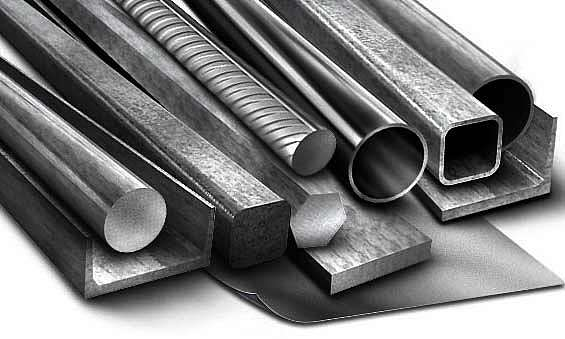
\includegraphics[height=0.4\textwidth]{pictures/steels}

\begin{itemize}
\item The most used material for machine components
\item It has been used for very long time, so behaviors are well understood
\item Compositions, thermal treatment and mechanical treatment can be used to obtain wide range of properties.
\end{itemize}
\end{frame}



\begin{frame}[label={sec:org24232ac}]{Basic Steel Selection Criteria\}}
\begin{itemize}
\item All steels have the same Young's moduli \(\rightarrow\) if stiffness is key, then choose the cheapest steel.
\item Carbon content determines the hardness. More carbon, harder steel.
\end{itemize}
\end{frame}



\begin{frame}[label={sec:org0cc5124}]{Heat Treatment of Steel Alloy\}}
\begin{itemize}
\item Parts can be heat-treated to obtain the same hardness with plain carbon steel as with more expensive alloys.
\item Alloying elements helps hardening. Hardness can be improved with less extreme heat treatments.
\end{itemize}

\vspace{0.3cm}
\centering
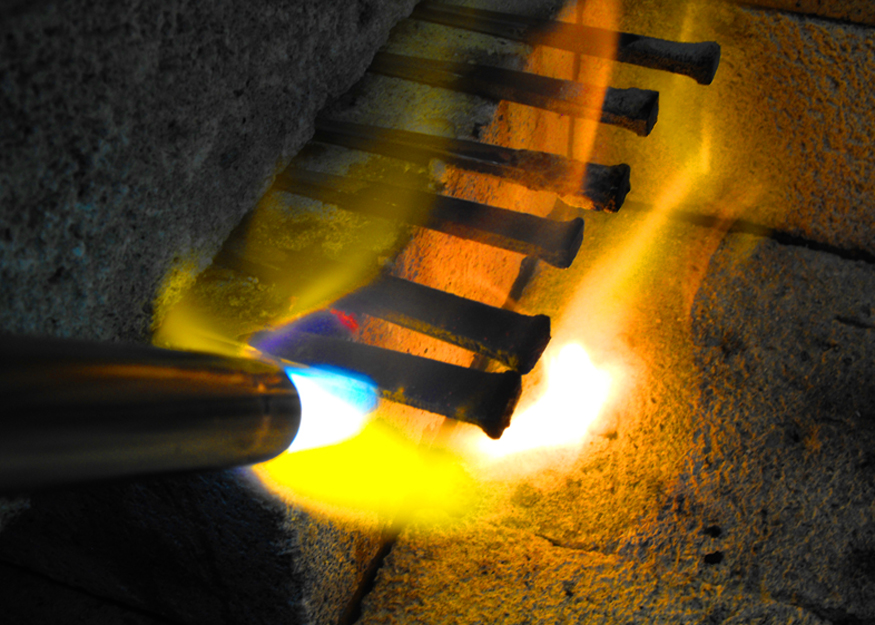
\includegraphics[height=0.4\textwidth]{pictures/heat-treatment}
\end{frame}



\begin{frame}[label={sec:org61e9918}]{Case-Hardening Steels\}}
Hardening of the surface, usually by carburizing, cyaniding, nitriding or induction hardening.

\begin{itemize}
\item Carburizing introduces additional carbon into steel and apply heat treatment.
\item Cyaniding introduces both carbon and nitrogen.
\item Nitriding adds nitrogen to the part surface at lower than 1000\(^{\circ}\) F or less so there is no risk of warpage.
\item Induction and flame hardening heat the surface then quench and temper.
\end{itemize}
\end{frame}

\begin{frame}[label={sec:orgeccbc03}]{Stainless Steels}
\centering
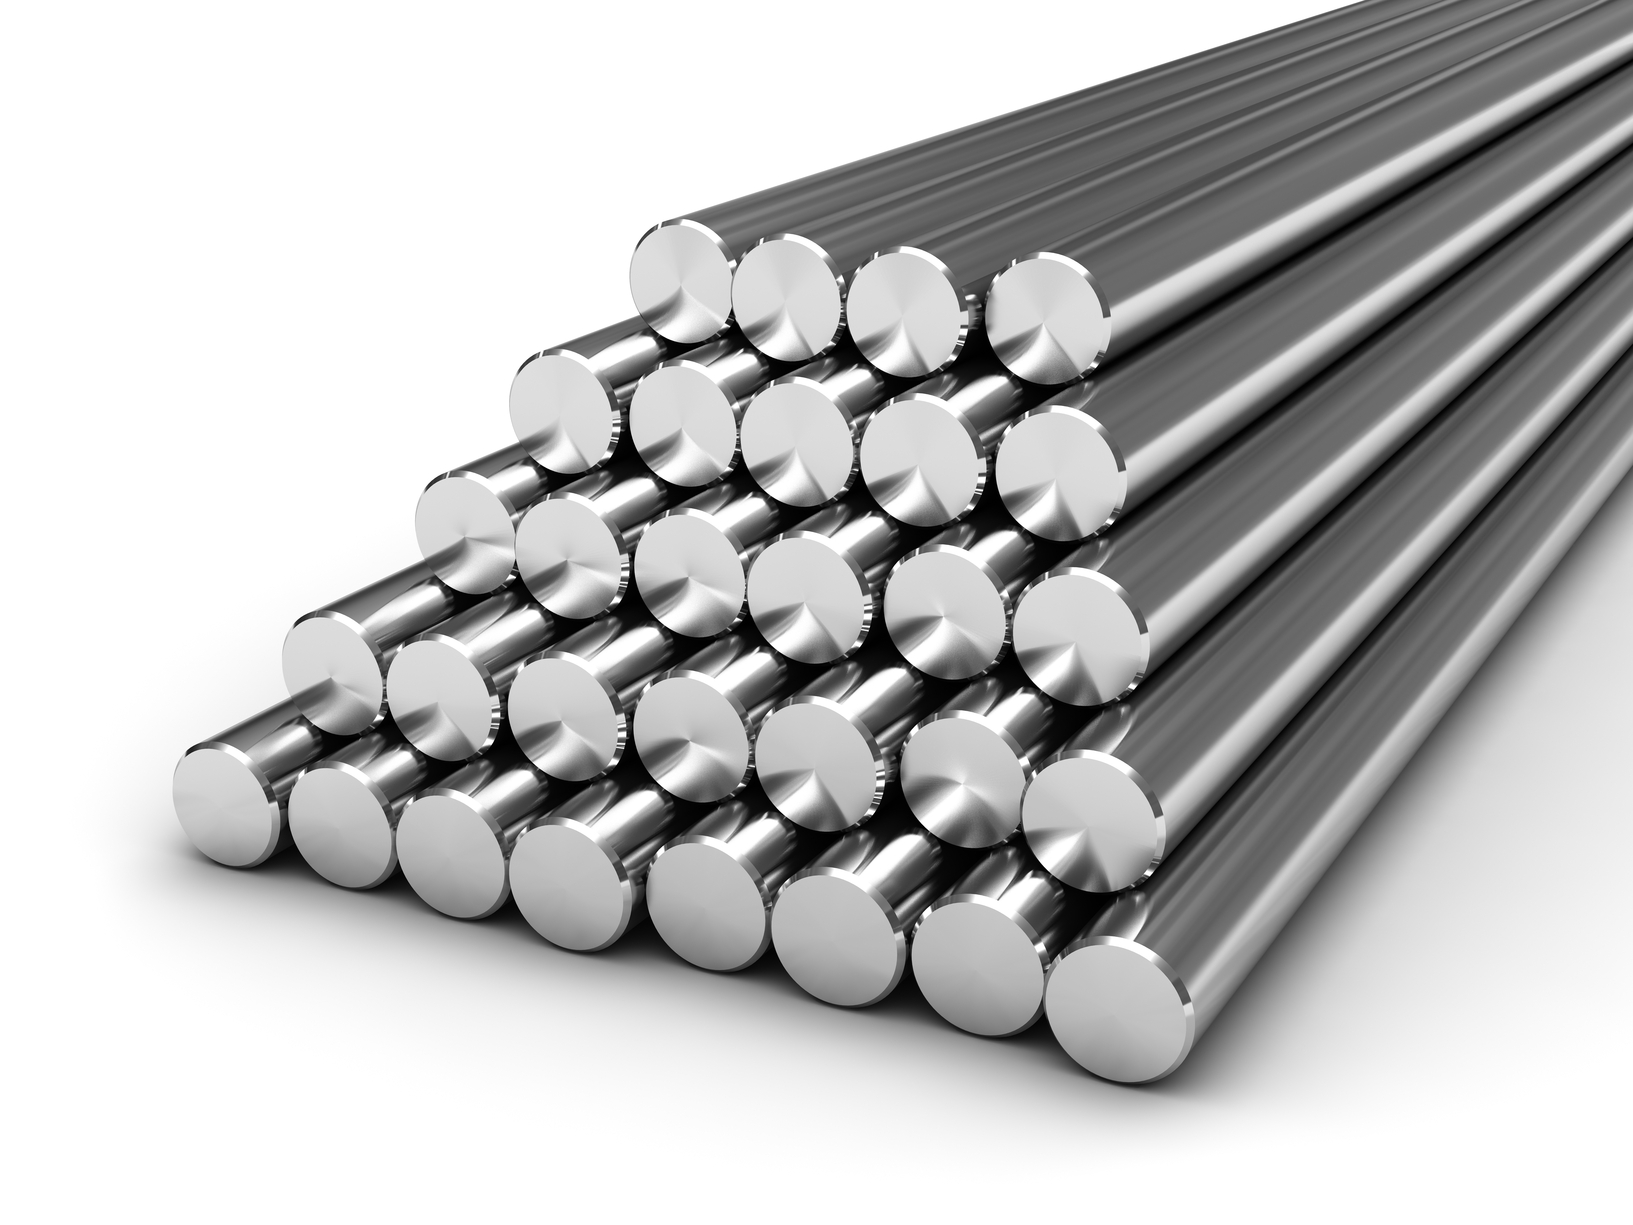
\includegraphics[height=0.5\textwidth]{pictures/stainless-steel}

\begin{itemize}
\item Contains a minimum of 10.5$\backslash$% chromium.
\item Heat-resistant and corrosion-resistant.
\item 3-5 times more expensive
\end{itemize}
\end{frame}

\begin{frame}[label={sec:org78257f7}]{Iron-based Superalloys}
\begin{itemize}
\item For high-temperature applications: gas turbines, jet engines, heat exchangers, furnaces \ldots{}
\item Strength at high temp and resistance to creep, corrosion, and wear.
\end{itemize}
\end{frame}

\begin{frame}[label={sec:org3cd870d}]{Aluminum Alloys}
\centering
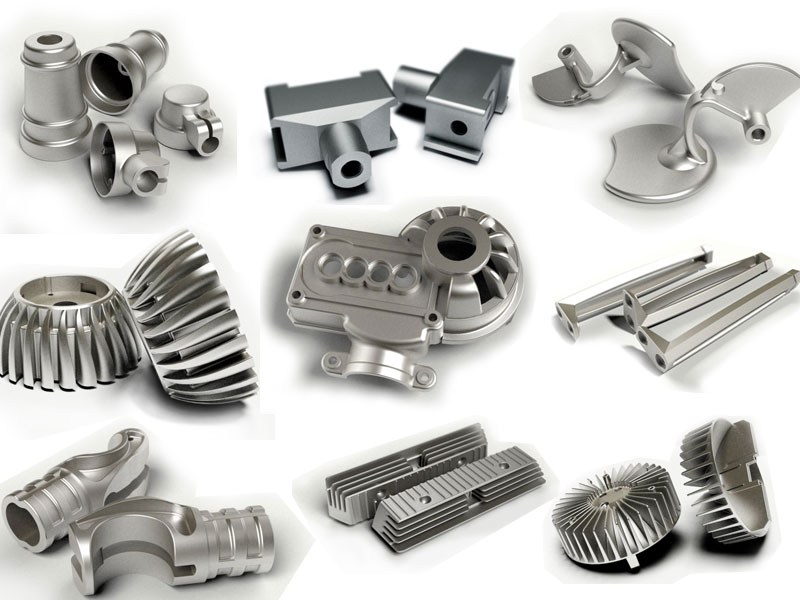
\includegraphics[height=0.4\textwidth]{pictures/aluminium-alloy}

\begin{itemize}
\item Slightly weaker but much lighter than steel
\item Difficult to harden
\item Lower geometric stabilility than steel.
\item Much easier to cast and machine.
\end{itemize}
\end{frame}

\begin{frame}[label={sec:org2602db6}]{Copper Alloy}
\begin{itemize}
\item Copper \& Brass
\item Excellent thermal and electrical conductivity. Good resistance to corrosion.
\item Poor strength.
\end{itemize}
\end{frame}

\begin{frame}[label={sec:org8aa5375}]{Other interesting alloys}
\begin{description}
\item[{Magnesium}] Lightest engineering metal.
\item[{Nickel}] strong and tough at extreme temperatures.
\item[{Titanium}] extremely corrosion-resistance, low thermal conductivity and good strength-weight ratio. Expensive and difficult to machine.
\item[{Zinc}] inexpensive. Easy to die-cast. Moderate strength.
\end{description}
\end{frame}


\begin{frame}[label={sec:org48ef63a}]{Overview of Plastics}
\begin{itemize}
\item Polymers form from small \emph{monomers}
\end{itemize}

\centering
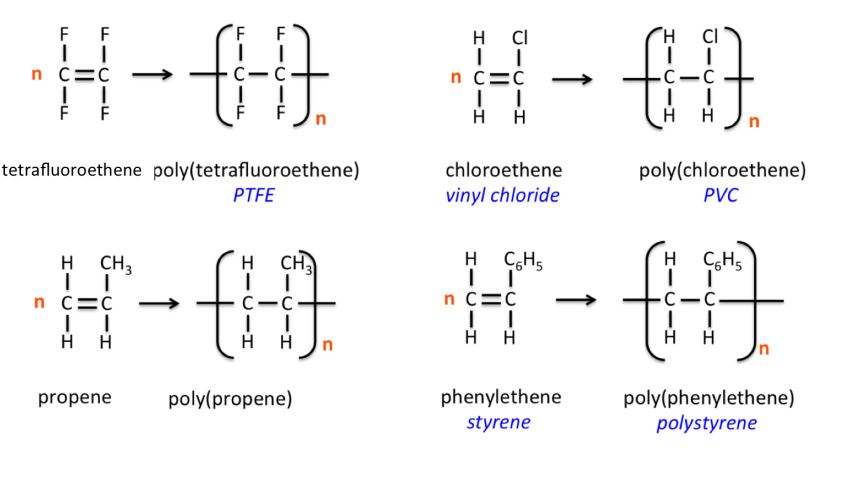
\includegraphics[width=0.9\textwidth]{pictures/polymer}
\end{frame}


\begin{frame}[label={sec:org6b76db4}]{Plastic Properties}
\begin{itemize}
\item More monomers \(\rightarrow\) heavier molecules \(\rightarrow\) gas, liquid, solid
\item Side branching leads to less packing and lower density, but also higher geometric stability and stiffness.
\item Divided on reaction to heat: thermoset (not softening) and thermoplastic (softening)
\end{itemize}
\end{frame}

\begin{frame}[label={sec:org58c806f}]{Thermoplastics}
\begin{description}
\item[{Polyester}] Excellent dimensional stability, electrical resistance, and toughness. Poor in outdoor and high temperature useage.
\item[{Polyethylene}] Lightweight. Easy to process. Inexpensive. Wide variety of grades from LDPE, MDPE, and HDPE. (Water bottle)

\centering
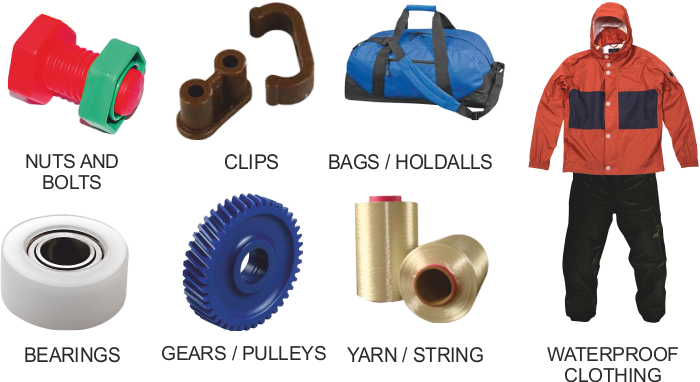
\includegraphics[width=0.45\textwidth]{pictures/nylon}
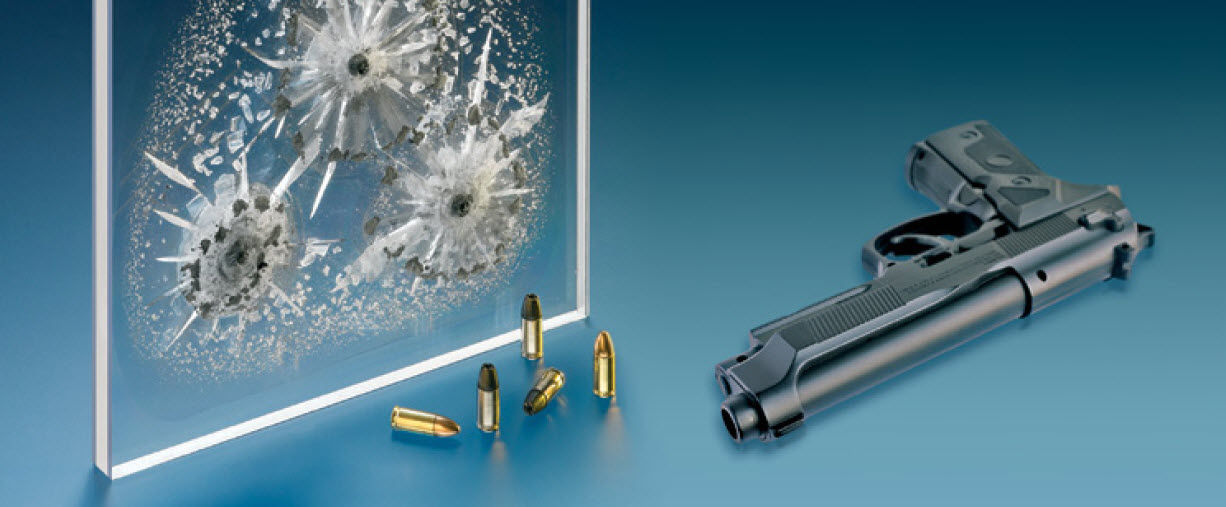
\includegraphics[width=0.45\textwidth]{pictures/polycarbonate} \\\empty
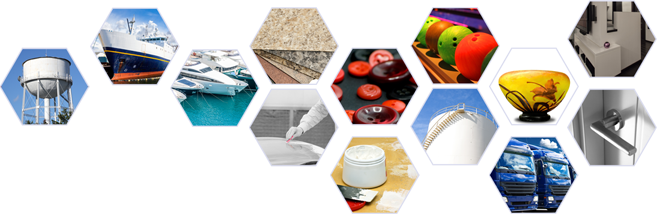
\includegraphics[width=0.45\textwidth]{pictures/polyester}
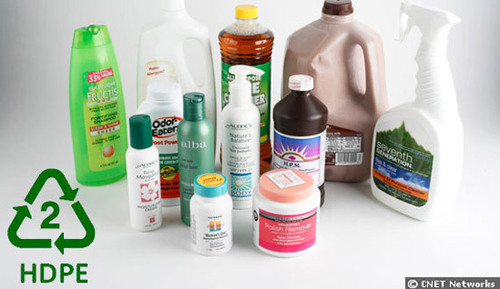
\includegraphics[width=0.45\textwidth]{pictures/HDPE}
\end{description}
\end{frame}


\begin{frame}[label={sec:orgd7e54a9}]{Thermoplastics II}
\begin{description}
\item[{Polypropylene}] Outstanding resistance to flex and stress cracking. Lightweight. Low cost. (Plastic bag)
\item[{Polystyrene}] Low-cost, clear, brittle. (Clear plastic box and covers.)
\item[{Polyurethane}] Tough, abrasion-resistant, and impact-resistant. (Resin floor coating)
\item[{PVC}] low cost. Many formulations available. Hard, tough, and good electrical resistance. Good outdoor stability and resistance to moisture.

\centering
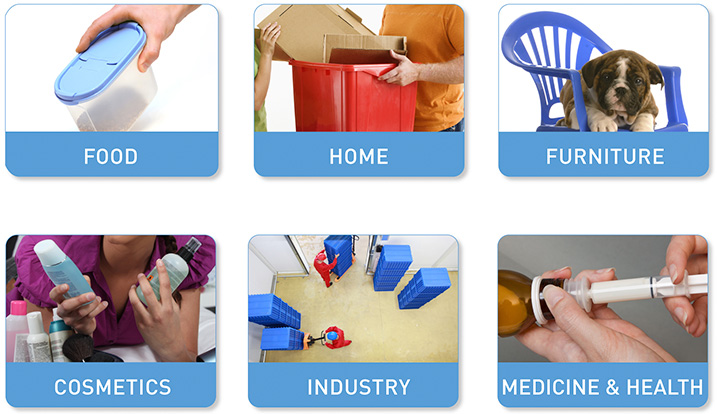
\includegraphics[width=0.45\textwidth]{pictures/polypropylene}
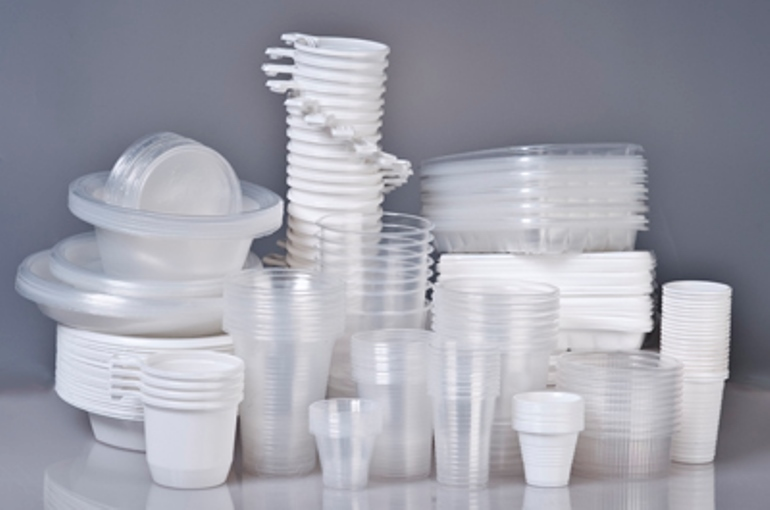
\includegraphics[width=0.45\textwidth]{pictures/polystyrene} \\\empty
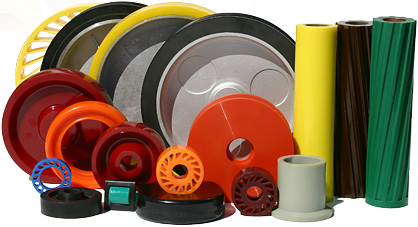
\includegraphics[width=0.45\textwidth]{pictures/polyurethane}
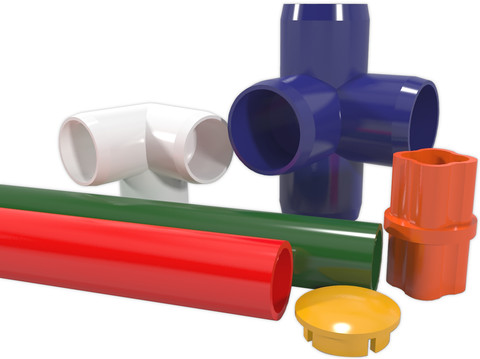
\includegraphics[width=0.45\textwidth]{pictures/pvc}
\end{description}
\end{frame}


\begin{frame}[label={sec:org5281fc4}]{Thermoset}
\begin{description}
\item[{Amino}] Abrasion and chip-resistant. Resistance to solvent. Melamine is hard and has high heat and chemical resistance.
\item[{Epoxy}] Exceptional mechanical strength and adhesion. (Epoxy glue)
\item[{Silicone}] Compatible with body tissue. High costs.

\centering
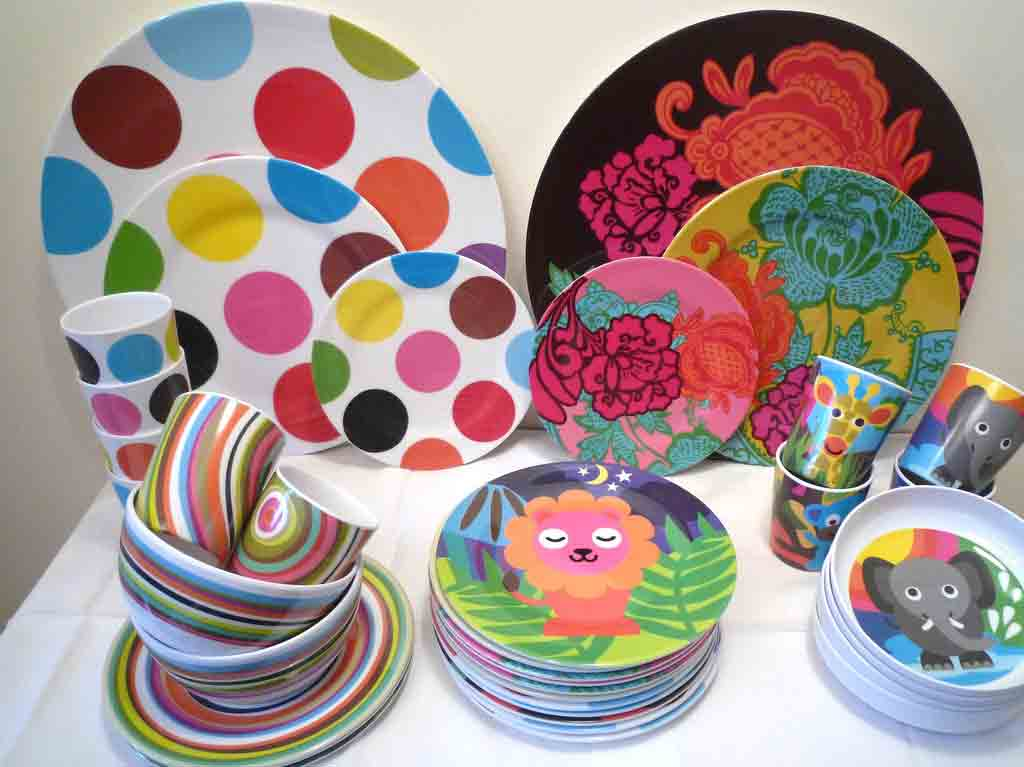
\includegraphics[width=0.4\textwidth]{pictures/melamine}
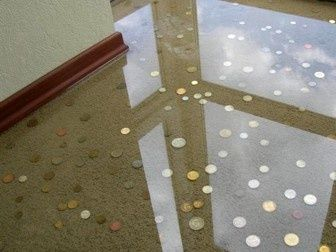
\includegraphics[width=0.4\textwidth]{pictures/epoxy}
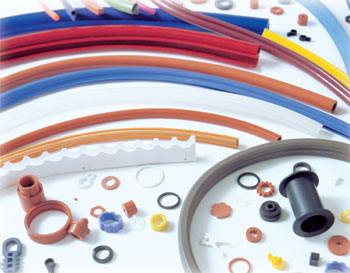
\includegraphics[width=0.4\textwidth]{pictures/silicone}
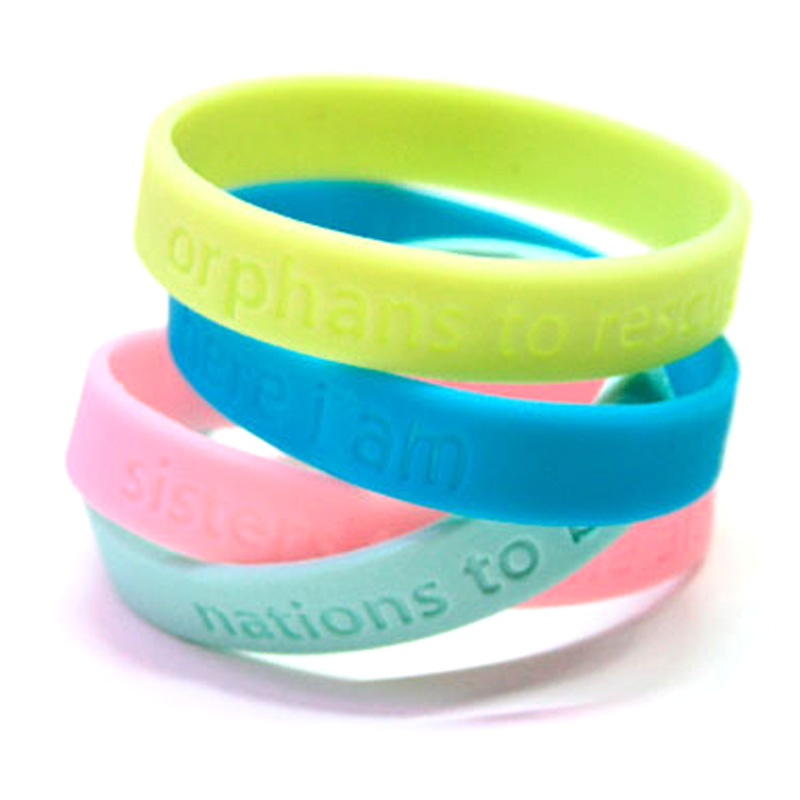
\includegraphics[width=0.3\textwidth]{pictures/silicone2}
\end{description}
\end{frame}


\begin{frame}[label={sec:orgb20b15d}]{Engineering Ceramics}
\centering
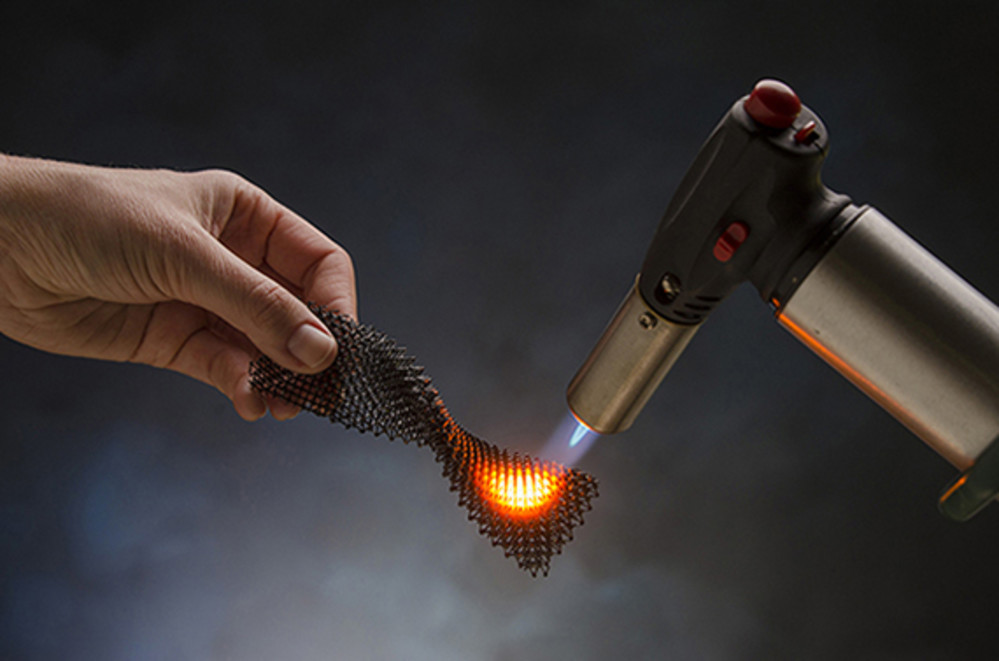
\includegraphics[height=0.5\textheight]{pictures/ceramic}

\begin{itemize}
\item Oxides, carbides, and nitrides
\item Extremely high temperature
\item High compressive strength, but brittle
\end{itemize}
\end{frame}

\begin{frame}[label={sec:org6e82fde}]{Examples of Engineering Ceramics}
\centering
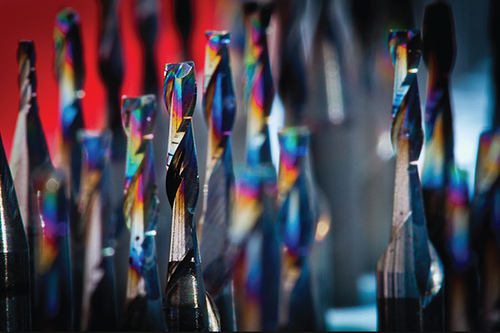
\includegraphics[width=0.4\textwidth]{pictures/diamond}
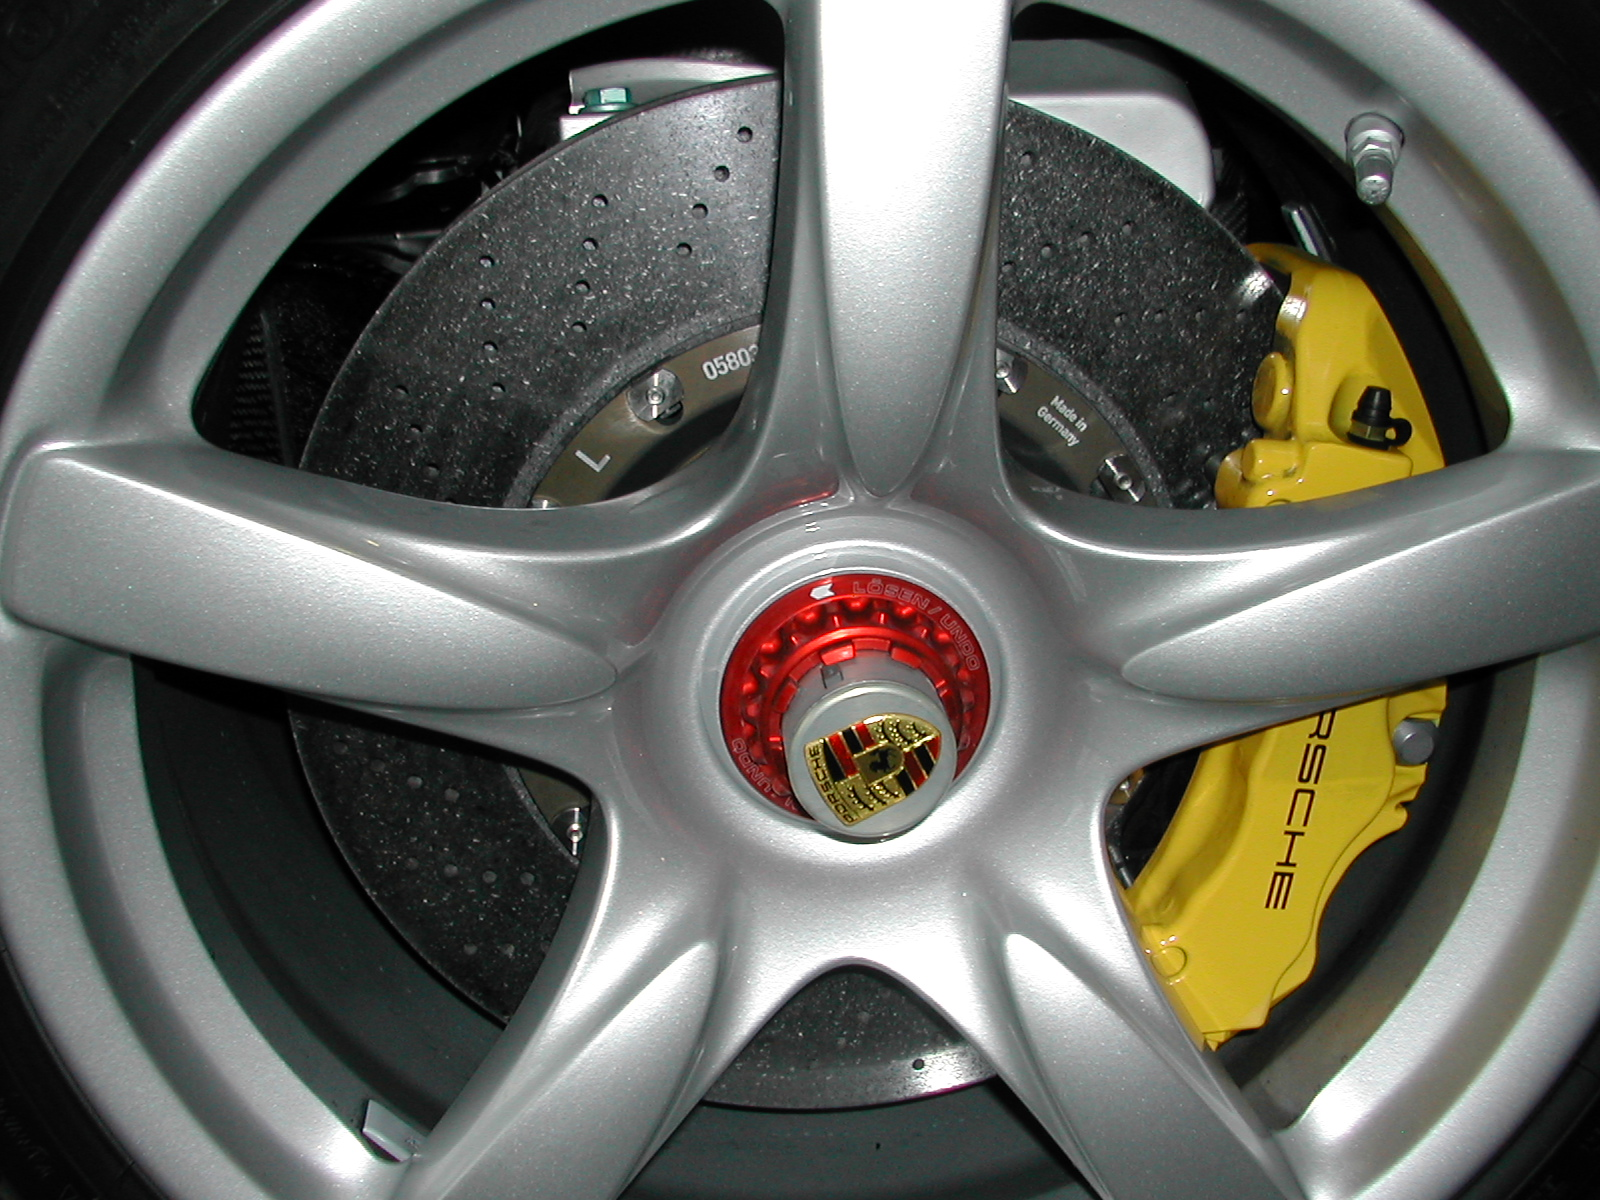
\includegraphics[width=0.4\textwidth]{pictures/silicon-carbide-disc-brake}
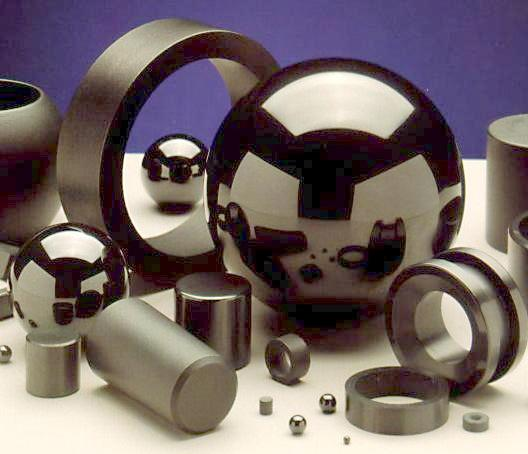
\includegraphics[width=0.4\textwidth]{pictures/silicon-nitride-bearing}
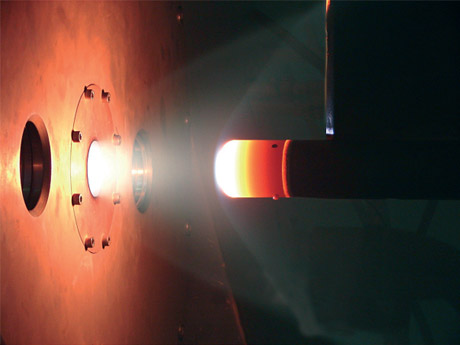
\includegraphics[width=0.4\textwidth]{pictures/ultra-high-temp}
\end{frame}


\begin{frame}[label={sec:org87434e0}]{Engineering Composites}
\begin{itemize}
\item Combine strengths of different materials.
\item CFRP, Steel-reinforced concrete, GFRP, etc.
\item Typically matrix + fibers
\end{itemize}

\centering
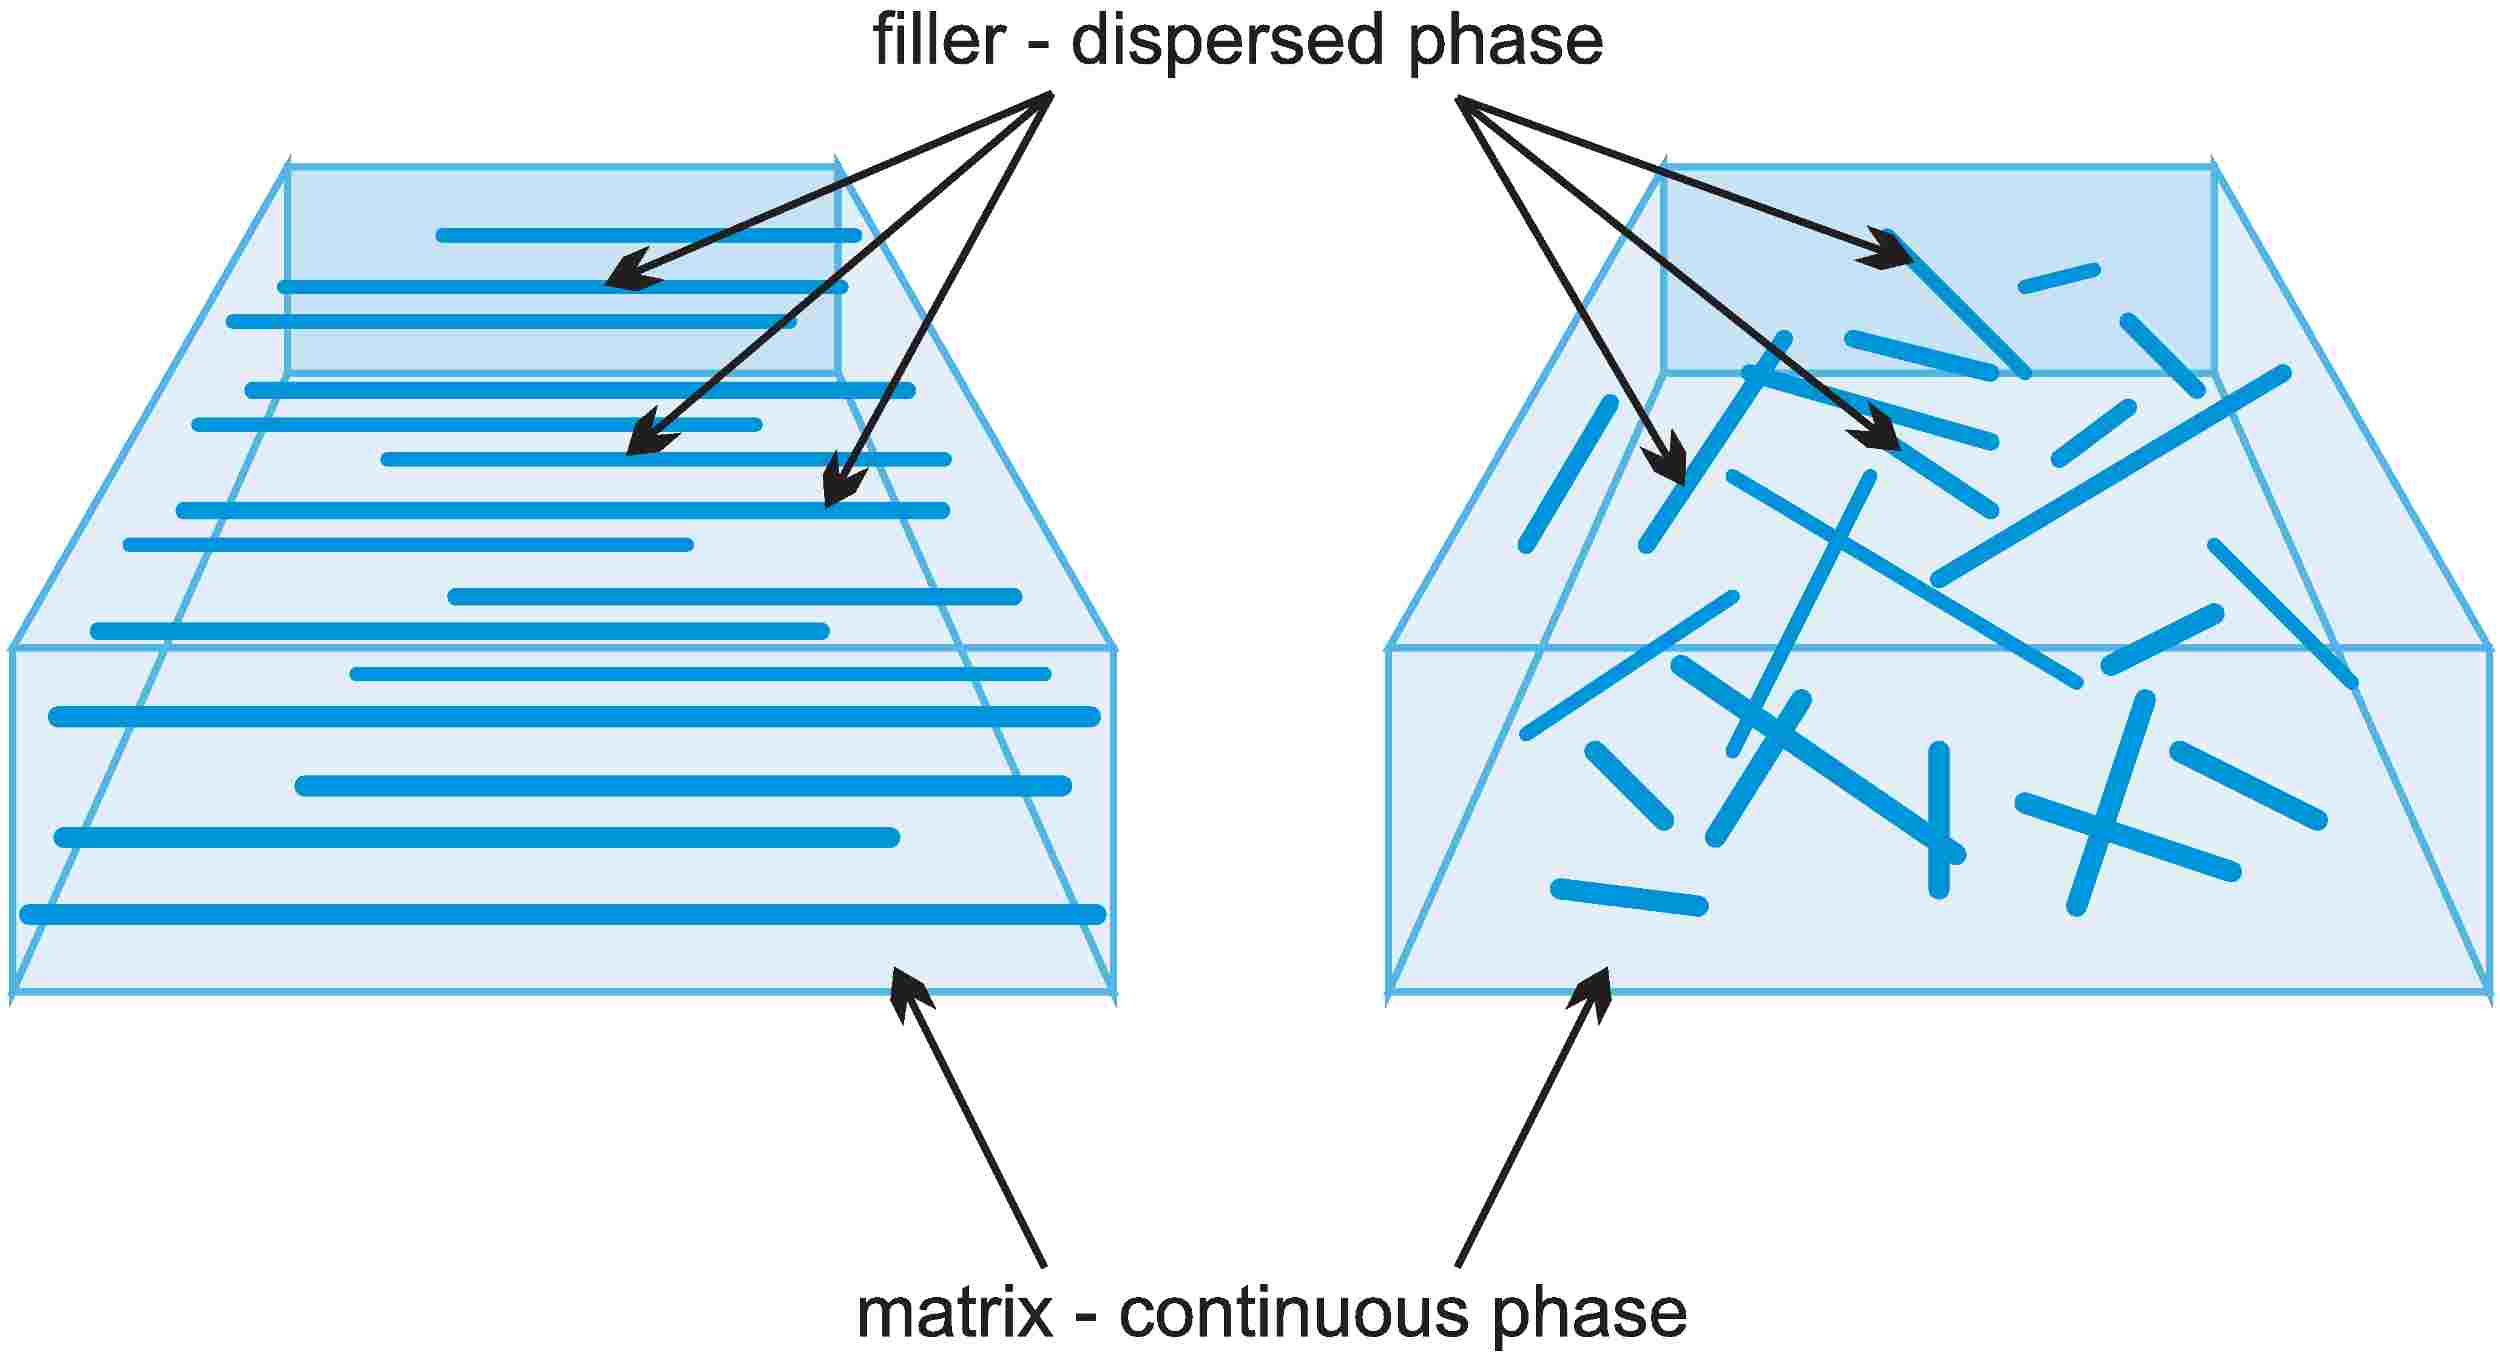
\includegraphics[height=0.4\textwidth]{pictures/matrix+fiber}
\end{frame}


\begin{frame}[label={sec:org65568a2}]{Examples of Composites}
\centering
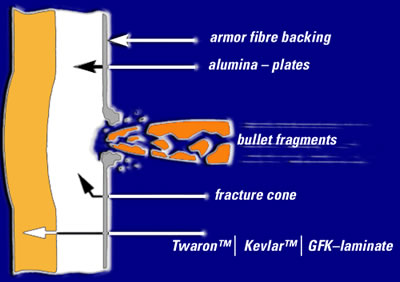
\includegraphics[width=0.4\textwidth]{pictures/composite-armor}
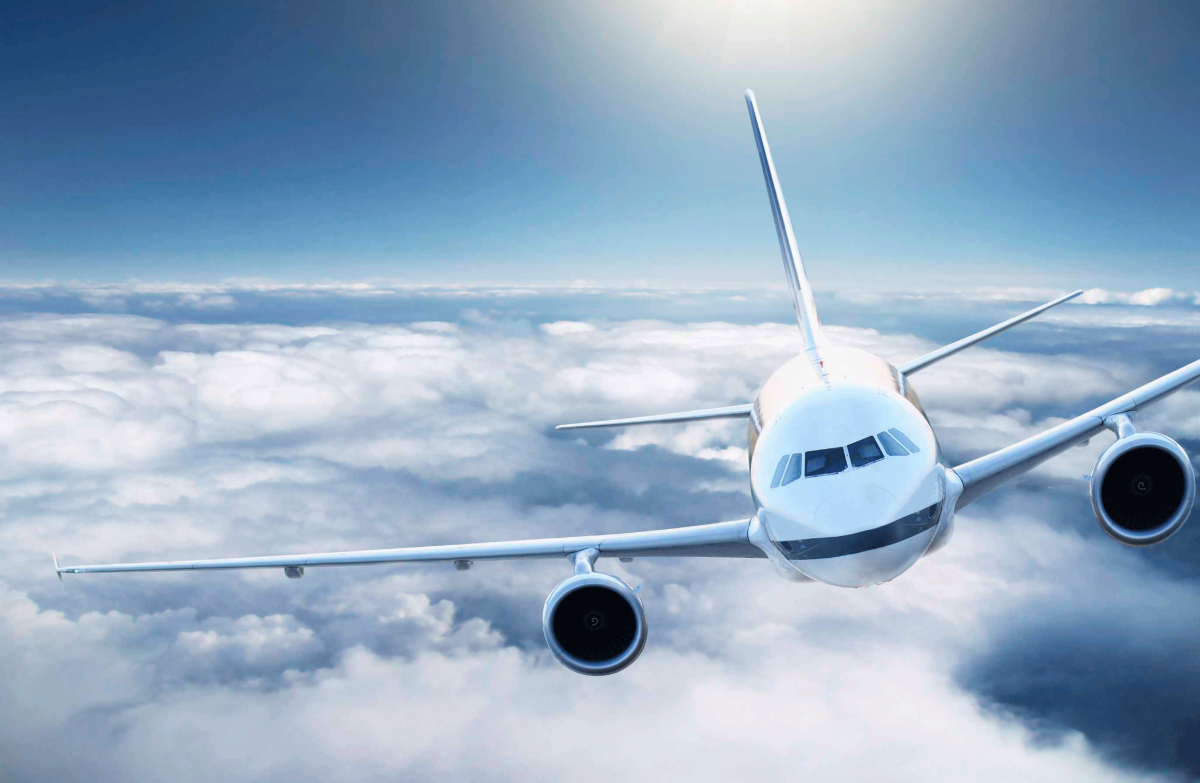
\includegraphics[width=0.4\textwidth]{pictures/application-aerospace1}
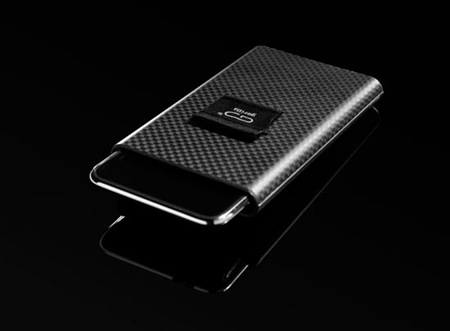
\includegraphics[width=0.4\textwidth]{pictures/cfrp-case}
\end{frame}

\section{Material Selection Considerations}
\label{sec:org54d714a}

\begin{frame}[label={sec:org82fa46e}]{Factors}
\begin{description}
\item[{Availability}] How easy it is to obtain or buy
\item[{Cost}] Raw material cost
\item[{Properties}] Strengths and weaknesses
\item[{Processes}] material - properties - processes are linked
\item[{Formability}] How easy it is to shape into desired components.
\item[{Finishing}] Enhance the properties for inexpensive materials.
\end{description}
\end{frame}

\begin{frame}[label={sec:org9e73606}]{Material Selection Charts}
\centering

\includegraphics[height=0.5\textheight]{pictures/wtf}

\begin{itemize}
\item Too many materials to browse through
\item Needs a way to quickly assess multiple material properties
\item Material selection charts!
\end{itemize}
\end{frame}



\begin{frame}[label={sec:orga498555}]{Material Selection Charts}
\begin{itemize}
\item Invented by M.F. Ashby in 1993, the charts map multiple materials together by their properties.
\item More details in \emph{Materials selection in mechanical design} (M. F. Ashby)
\item Bubble charts and bar charts
\end{itemize}

\centering
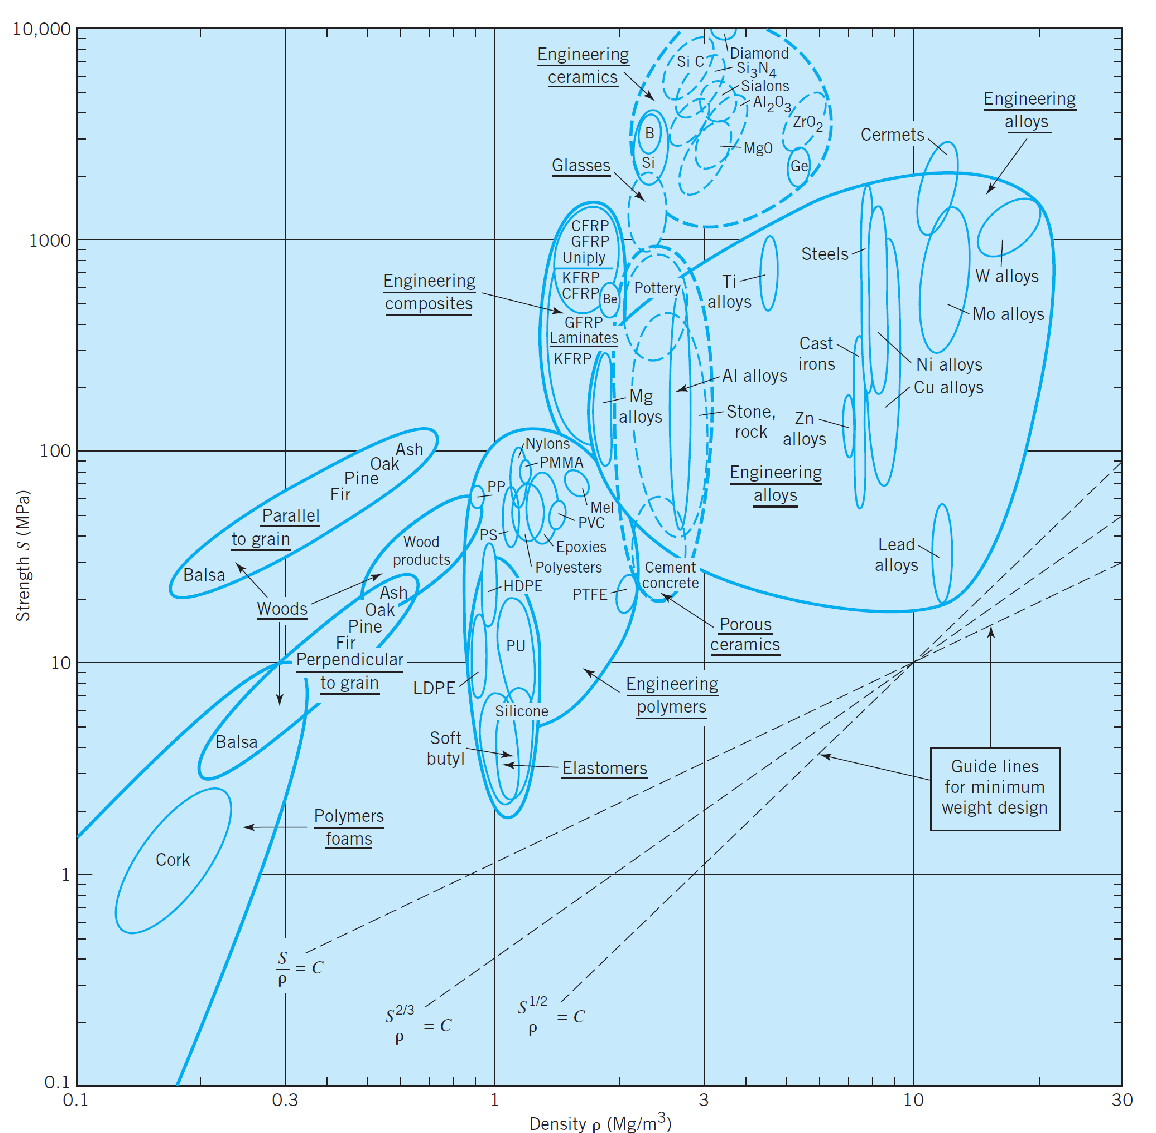
\includegraphics[height=0.5\textheight]{pictures/strength-density-diagram}
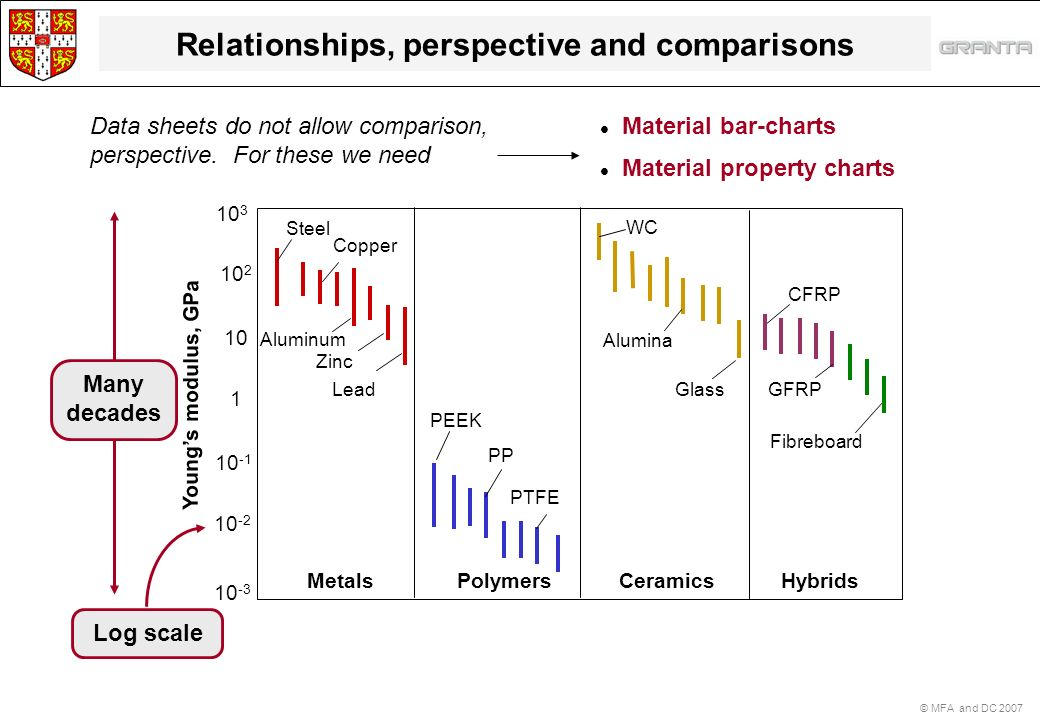
\includegraphics[height=0.5\textheight]{pictures/mat-bar-chart}
\end{frame}


\section{Material Selection Procedure}
\label{sec:org66f69b0}

\begin{frame}[label={sec:org0df80a8}]{The procedure}
\begin{itemize}
\item Establish required service performances
\item Select a suitable material
\item Make a final evaluation
\item Test, a lot of tests
\end{itemize}
\end{frame}



\begin{frame}[label={sec:org8251655}]{Establish Required Performance}
\begin{itemize}
\item Determine the operational conditions of the component
\item Translate into material properties.
\end{itemize}

\vspace{1cm}
\centering
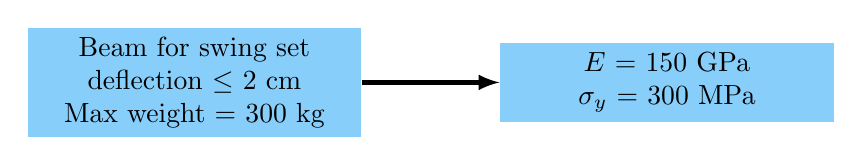
\begin{tikzpicture}[>=latex, every node/.style={fill=LightSkyBlue}]
  \node [text width=4cm, align=center](A){Beam for swing set \\ deflection $\leq$ 2 cm \\ Max weight = 300 kg};
  \node [text width=4cm, align=center, xshift=6cm](B){$E$ = 150 GPa \\ $\sigma_y$ = 300 MPa};
  \draw [ultra thick, ->] (A) -- (B);
\end{tikzpicture}
\end{frame}


\begin{frame}[label={sec:orgae5d983}]{Select a Suitable Material\}}
\centering
\begin{tikzpicture}
  \clip (-4.1,-3) rectangle ++(9,5);
  \node{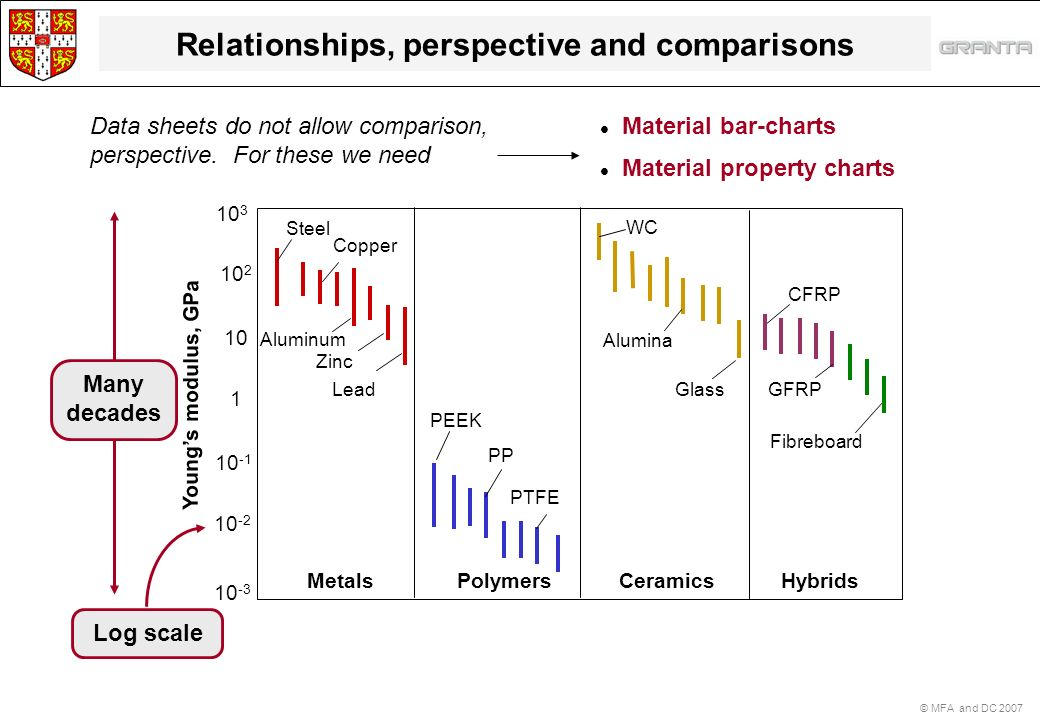
\includegraphics[height=\textheight]{pictures/mat-bar-chart}};
\end{tikzpicture}

\begin{itemize}
\item Looking through data sheets is not fun
\item Material charts are much better
\end{itemize}
\end{frame}



\begin{frame}[label={sec:orgc94adb2}]{Make a Final Evaluation\}}
\begin{itemize}
\item Select the best material for the application
\item `Best' is the material with the best value, defined simply as the material selection index (SI) where
$$ SI = \frac{(\text{availability})(\text{performance})}{\text{total cost}} $$
\end{itemize}
\end{frame}



\begin{frame}[label={sec:org8ccce44}]{Test, test, and more test\}}
\begin{itemize}
\item Test in operating conditions.
\item Do we need more tests?
\item Reevaluate the risk and uncertainty of chosen material, for example, cost of product failure.
\end{itemize}

\centering
\begin{tikzpicture}
  \clip (-4.1,-2) rectangle ++(9,4);
  \node{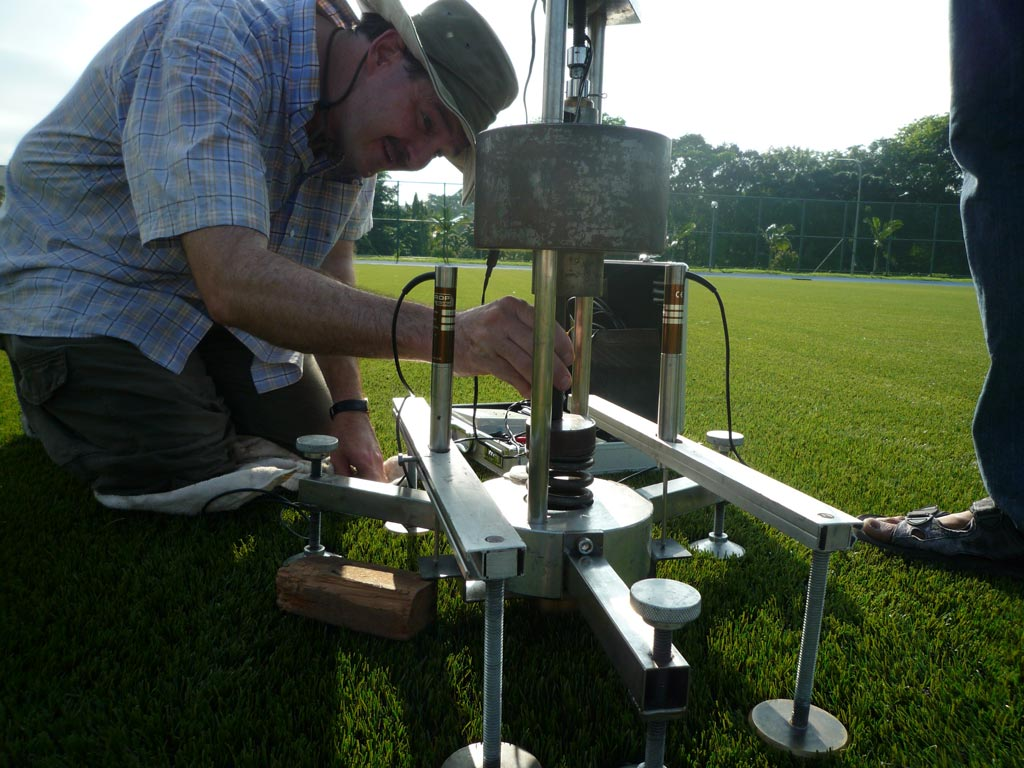
\includegraphics[height=0.6\textheight]{pictures/field-test}};
\end{tikzpicture}
\end{frame}


\begin{frame}[label={sec:org4868795}]{Example: Minimum Weight Bar\}}
Design a lightest possible tensile bar that can take \(F_{\max} = 50000 \text{ N}\). We have 3 material choices.
\vspace{5mm}

\centering
\begin{tabular}{lcc}
  \toprule
  Material & Density & Yield Strength \\
  \midrule
  HSS    & 7800    & 1200 \\
  Aluminum & 2300    & 400 \\
  CFRP     & 1500    & 350 \\
  \bottomrule
\end{tabular}
\end{frame}


\begin{frame}[label={sec:orgfac73f3}]{The Hard Way}
Let's assume \(N_s = 2\). The cross-sectional area required for each material is

\begin{gather*}
  N_s = \frac{S_y}{\dfrac{F}{A}} \\
  A = \frac{N_S F}{S_y}
\end{gather*}

\begin{center}
\begin{tabular}{lc}
\toprule
HSS & 8.33e-05 m$^2$ \\
Aluminum & 2.50e-04 m$^2$ \\
CFRP & 2.86e-04 m$^2$ \\
\bottomrule
\end{tabular}
\end{center}
\end{frame}


\begin{frame}[label={sec:orgfe34afd}]{Comparing mass}
Once cross-sectional areas are obtained, mass is just

\begin{equation*}
  m = \rho A l
\end{equation*}

\begin{center}
\begin{tabular}{lc}
\toprule
Material & Mass (kg) \\
\midrule
HSS & 6.50e-01 $l$ \\
Aluminum & 5.75e-01 $l$ \\
CFRP & 4.29e-01 $l$ \\
\bottomrule
\end{tabular}
\end{center}

So CFRP is the lightest, regardless of length \(l\).
\end{frame}


\begin{frame}[label={sec:orgca43657}]{The `Easy' Way}
Combine the equations for area and mass

\begin{align*}
  m &= \rho A l \\
    &= \rho N_s \frac{F}{S_y} l
\end{align*}

Well, \(N_s\), \(F\), and \(l\) are all given by the problem
\end{frame}


\begin{frame}[label={sec:org1de6672}]{Strength - Weight Ratio}
We simply need to determine a single ratio
\begin{gather*}
  m \sim \frac{\rho}{S_y}
\end{gather*}

to identify the lightest material for the application
\end{frame}



\begin{frame}[label={sec:orgf93f10e}]{Minimum weight index}
Guideline for strength-based minimum weight design

\centering
\begin{tabular}{l c}
  \toprule
  Load condition & Min weight index \\
  \midrule
  Tension & $\dfrac{S_y}{\rho}$ \\[10pt]
  Bending, torsion & $\dfrac{S_y^{2/3}}{\rho}$ \\[10pt]
  Plate under normal load & $\dfrac{S_y^{1/2}}{\rho}$ \\
  \bottomrule
\end{tabular}
\end{frame}


\begin{frame}[label={sec:org605081c}]{Example: Material for a Gas Turbine Shaft}
\centering
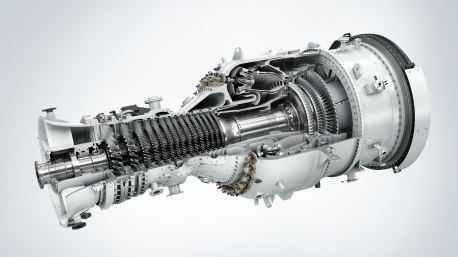
\includegraphics[width=0.5\textwidth]{pictures/gas-turbine-shaft}

\begin{itemize}
\item What material properties should be considered?

\pause - mass / density
\pause - strength
\pause - temperature
\pause - cost
\end{itemize}
\end{frame}

\begin{frame}[label={sec:org13b7044}]{Establish required performances}
\begin{itemize}
\item Shaft as light as possible
\item Operating temperature \$> 300\textsuperscript{\^{}}\$C
\item Cost is not a concern
\end{itemize}
\end{frame}



\begin{frame}[label={sec:org6c7bf45}]{Establish required performances}
\begin{itemize}
\item Shaft as light as possible \(\rightarrow\) strength - density diagram
\item Operating temperature \$> 300\textsuperscript{\^{}}\$C \(\rightarrow\) strength - temp diagram
\item Cost is not a concern \(\rightarrow\) yay?
\end{itemize}
\end{frame}



\begin{frame}[label={sec:org71a2332}]{Can you stand the heat?}
\centering
\begin{tikzpicture}[>=latex]
  \node(A){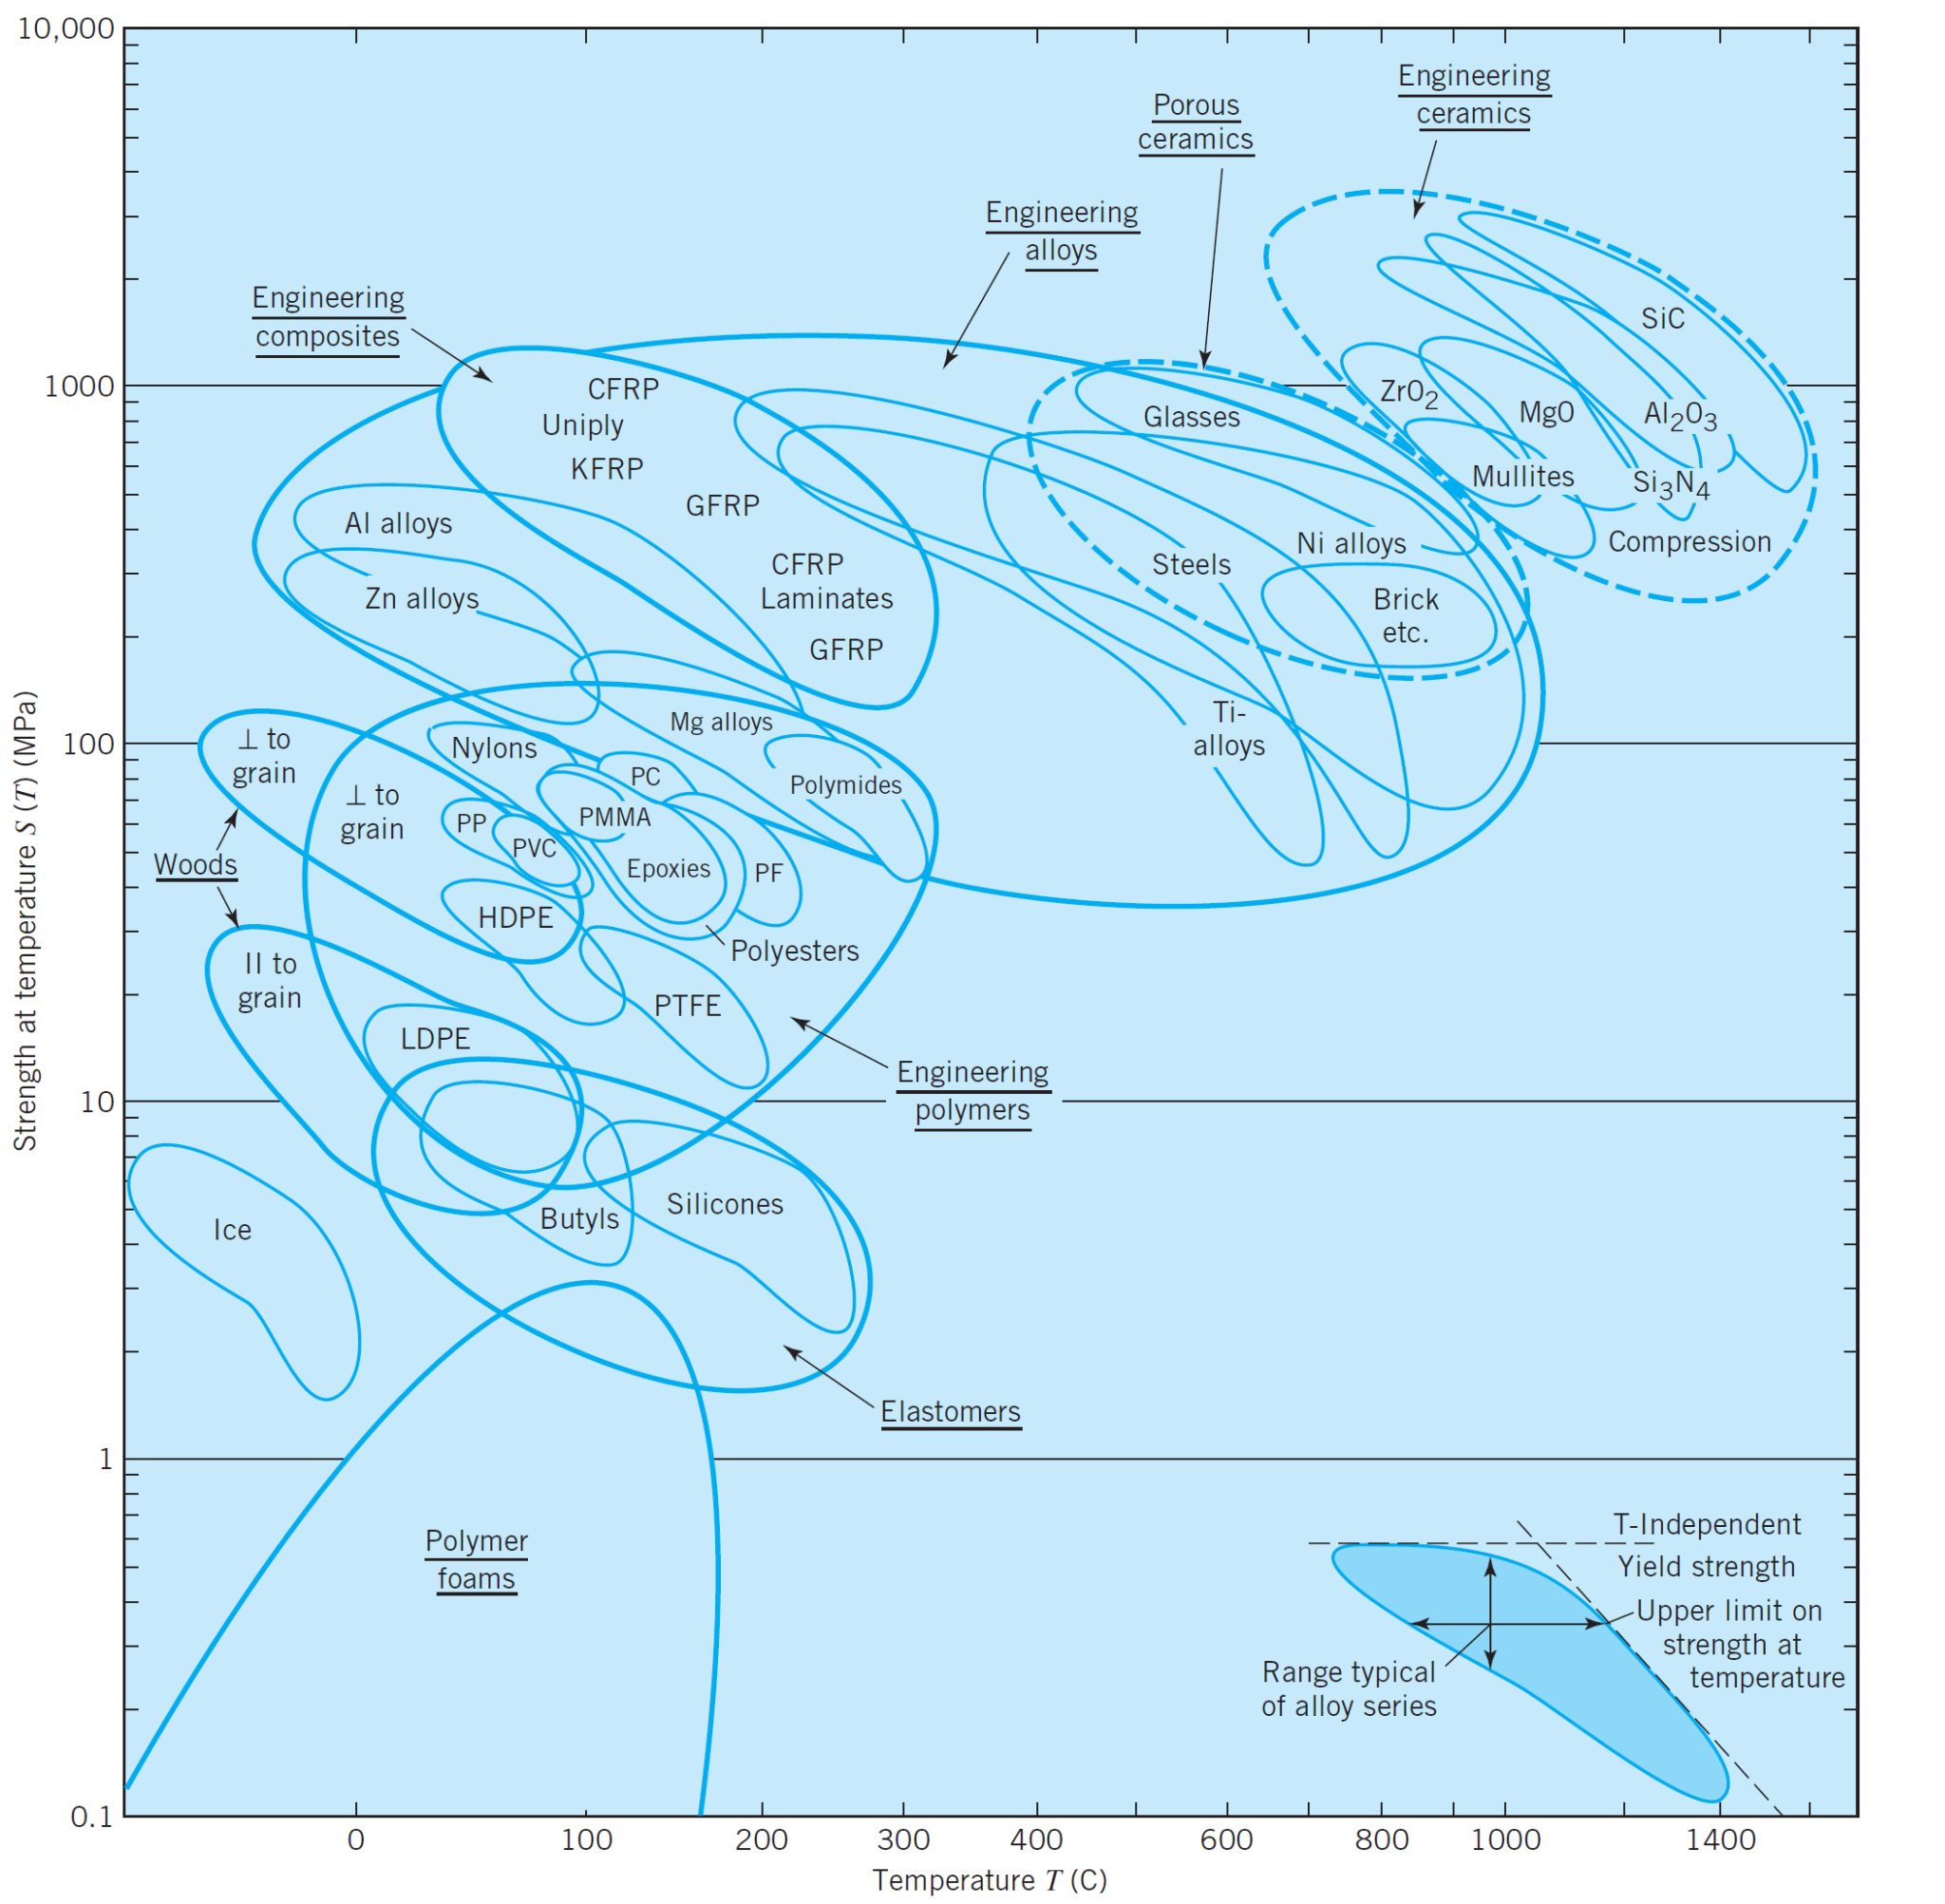
\includegraphics[height=0.8\textheight]{pictures/strength-temperature-diagram}}; \pause
  \draw [dashed, red] (A.south) ++ (180:0.25) --++ (90:7.5) node[midway, left, red]{300 C}; \pause
  \node at (A.north east) [xshift=-2cm, yshift=-2cm, circle, draw, red, minimum height=2.5cm](C){};
  \node at (C.south) [below, Blue, text width=3cm, align=center]{Metal alloys and ceramics};
\end{tikzpicture}
\end{frame}


\begin{frame}[label={sec:orgc446b4f}]{Minimize the weight}
\centering
\begin{tikzpicture}[>=latex]
  \node(A){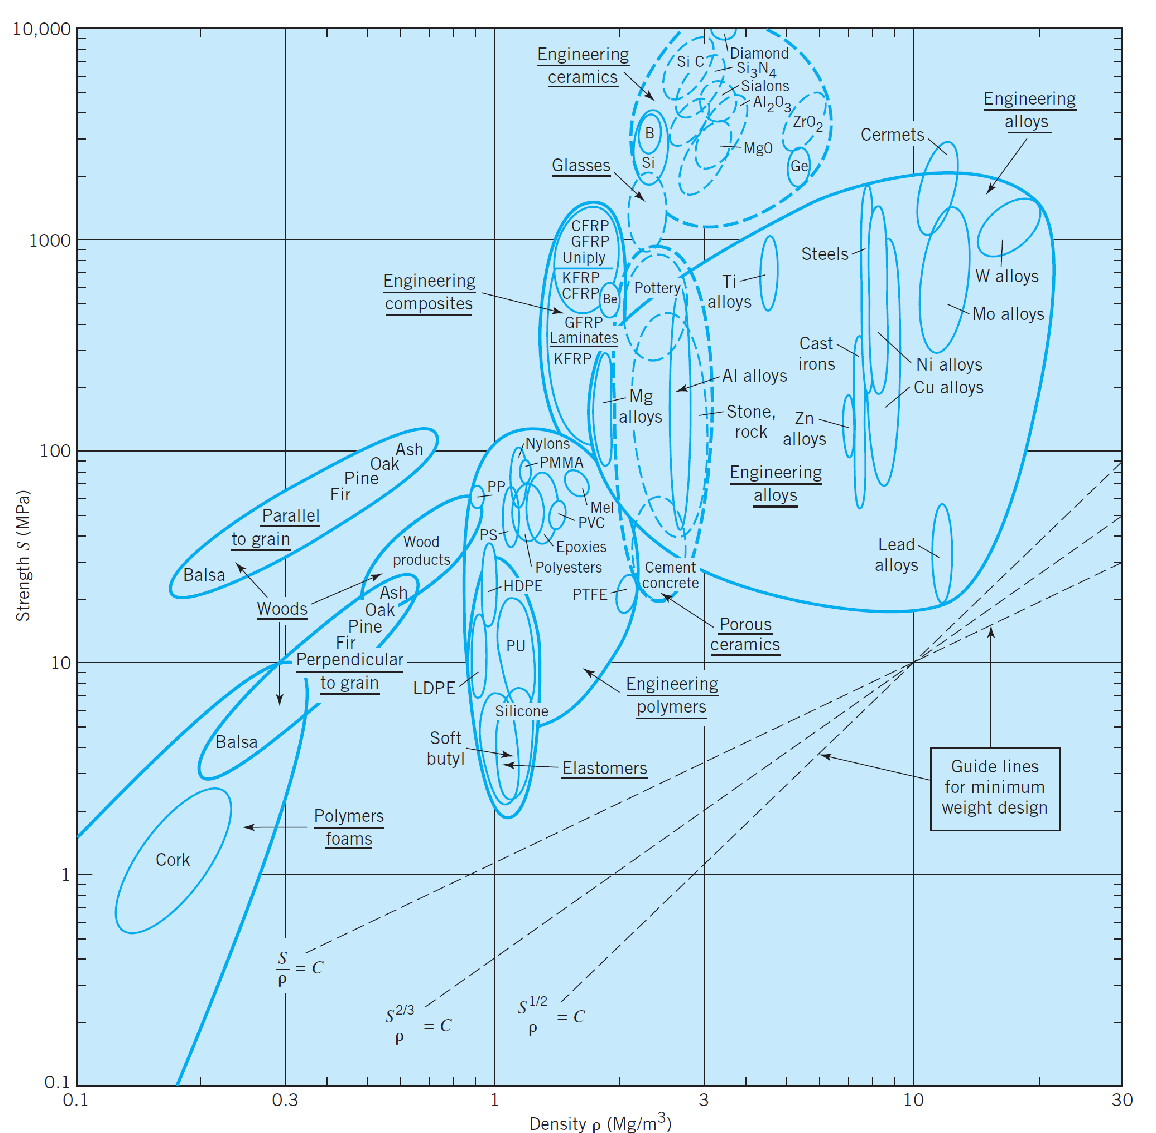
\includegraphics[height=0.8\textheight]{pictures/strength-density-diagram}};
  \only<1> {
    \draw [dashed, red] (A.east) ++ (90:0.55) --++ (-145:6) node[midway, right, red]{$\dfrac{S^{2/3}}{\rho} = C_1$};
  }
  \only<2> {
    \draw [->, red] (A.south east) ++ (135:3.5) --++ (135:3);
    \draw [dashed, red] (A.north) ++ (0:1.3) --++ (-145:6) node[midway, above, red]{$\dfrac{S^{2/3}}{\rho} = C_2$};
  }
\end{tikzpicture}
\end{frame}


\begin{frame}[label={sec:org42cc864}]{Combine the results}
\begin{itemize}
\item Light shaft \(\rightarrow\) ceramics, woods // to grains, composites, and metal alloys
\item High temperature operation NOT OK \(\rightarrow\) woods, composites, Zn, Al, and Mg alloys
\item Preliminary choices \(\rightarrow\) ceramics, Ti, Ni, and Steel alloys
\end{itemize}
\end{frame}



\begin{frame}[label={sec:orgdebd44d}]{Additional evaluations}
\begin{itemize}
\item 1st choice - ceramics

\begin{itemize}
\item Hard to machine
\item Brittle
\end{itemize}

\item 2nd choice - Ti, Ni, or Steels
\item Test (simulation or prototype) to obtain final choice
\end{itemize}

\centering
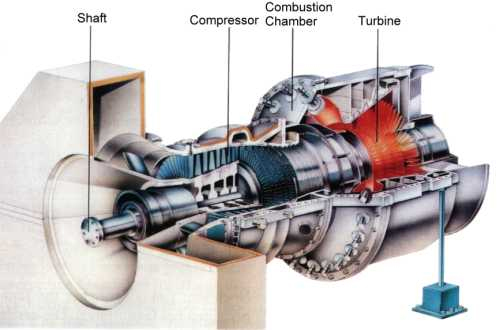
\includegraphics[height=0.5\textheight]{pictures/turbine-shaft}
\end{frame}


\begin{frame}[label={sec:orga759102}]{}
\Huge\centering Any Questions?
\end{frame}
\end{document}